\documentclass[a4paper, 12pt, twoside]{article}
\usepackage{estilo}

% ── Margens laterais estritamente oficiais (2.5cm) conforme edital EU ──
\geometry{
  a4paper,
  inner=2.5cm, outer=2.5cm,
  top=2.0cm, bottom=1.5cm,
  headheight=40pt, headsep=12pt
}
\setstretch{0.86}
\setlength{\parindent}{0.70cm}
\setlength{\textfloatsep}{2pt plus 1pt minus 1pt}
\setlength{\intextsep}{2pt plus 1pt minus 1pt}
\setlength{\abovecaptionskip}{1.5pt}
\setlength{\belowcaptionskip}{1.5pt}

\title{Redes Neurais Informadas por Física em Domínios Irregulares: Análise Comparativa frente ao Método ADI na Equação do Calor 2D}

\author{%
  G. Warley B. Farias\authorinfo{warrley@alu.ufc.br} \\
  R. Reis Pereira\authorinfo{reis@ufc.br}
}
\date{}

\begin{document}
\maketitle

%%%%%%%%%%%%%%%%%%%%% RESUMO E ABSTRACT %%%%%%%%%%%%%%%%%%%%%%%%%%%%%%

\qabstract{Resumo}{Palavras-chave}{ODS}{%
A simulação da condução térmica transiente em sólidos com domínios irregulares e múltiplos sumidouros perfurados impõe severos desafios aos esquemas numéricos clássicos. O Método de Diferenças Finitas (MDF) com Direções Alternadas Implícitas (ADI), formalizado por \textcite{pereira2019}, exibe custo computacional linear ótimo $\mathcal{O}(N)$ em malhas regulares, mas sofre degradação pelo erro de escadeamento (\textit{staircasing}) e quebra da tridiagonalidade em contornos curvos. Este trabalho investiga as Redes Neurais Informadas por Física (PINNs) como um resolvedor contínuo e livre de malha (\textit{meshless}) para a Equação do Calor 2D em um domínio multiconectado com três cavidades circulares dissipadoras. A topologia geométrica é assimilada no funcional de perda via diferenciação automática (\textit{autograd}). Após 50.000 épocas Adam, a PINN atinge erro residual de $2{,}43 \times 10^{-6}$ nas barreiras de Dirichlet dos furos, superando descontinuidades de malha. Analisam-se a rigidez de gradiente (\textit{stiffness}) na época 26.000, o relevo térmico tridimensional nas cavidades e as limitações da inferência global espaço-temporal frente à marcha causal sequencial de \textcite{pereira2019}.%
}{%
redes neurais informadas por física; equação do calor; método de diferenças finitas; direções alternadas implícitas; erro de escadeamento%
}{%
indústria, inovação e infraestrutura%
}

\qabstract{Abstract}{Keywords}{SDG}{%
Transient heat conduction in solid media with irregular domains and perforated cooling cavities imposes severe challenges on classical numerical schemes. The Finite Difference Method (FDM) based on the Alternating Direction Implicit (ADI) scheme, formalized by \textcite{pereira2019}, achieves optimal $\mathcal{O}(N)$ complexity on regular grids, but suffers from staircasing errors and breakdown of tridiagonal factorization on curved boundaries. This work investigates Physics-Informed Neural Networks (PINNs) as a continuous, mesh-free solver for the 2D heat equation in a multiply connected domain containing three circular cooling cavities. Boundary manifolds are analytically assimilated into a weighted multi-objective loss function via automatic differentiation. After 50,000 Adam epochs, the PINN enforces Dirichlet sink boundaries with residual errors of $2.43 \times 10^{-6}$, completely circumventing grid artifacts. We analyze the gradient stiffness pathology at epoch 26,000, examine the continuous three-dimensional thermal relief inside cavities, and evaluate global space-time block optimization versus the causal marching of \textcite{pereira2019}.%
}{%
physics-informed neural networks; heat equation; finite difference method; alternating direction implicit; staircasing error%
}{%
industry, innovation and infrastructure%
}

%%%%%%%%%%%%%%%%%%%%%%%%%%%%%% SEÇÕES %%%%%%%%%%%%%%%%%%%%%%%%%%%%%

\section{Introdução}

A modelagem quantitativa da difusão térmica transiente em domínios espaciais multiconectados desempenha papel fulcral no projeto de trocadores de calor, sistemas microeletromecânicos e gerenciamento térmico de circuitos integrados com múltiplos canais dissipadores. Historicamente, o \textbf{Método de Diferenças Finitas (MDF)} consolidou-se como ferramenta preponderante para a integração temporal de \textbf{Equações Diferenciais Parciais (EDPs)} parabólicas, impulsionado pelo consagrado esquema de \textbf{Direções Alternadas Implícitas (ADI)} de \textcite{peaceman1955}, cujos fundamentos teóricos e estabilidade numérica foram formalizados para problemas não lineares de transporte e reação-difusão na tese de \textcite{pereira2019}.

Em geometrias cartesianas retangulares uniformes, o método ADI decompõe o operador Laplaciano bidimensional em passos unidimensionais implícitos sucessivos de meia etapa temporal. Essa formulação desacopla as coordenadas espaciais em sistemas tridiagonais estritamente diagonais dominantes, resolvidos pelo Algoritmo de Thomas com complexidade linear $\mathcal{O}(N)$ e estabilidade incondicional de von Neumann \parencite{peaceman1955, pereira2019}.

No entanto, a eficiência matricial do ADI cessa diante de geometrias com contornos curvos ou não ortogonais. Em grades cartesianas, a representação de superfícies radiais induz o \textbf{erro de escadeamento (\textit{staircasing})}, aproximando contornos suaves por degraus ortogonais descontínuos. Essa discretização espúria introduz um erro geométrico de truncamento de primeira ordem $\mathcal{O}(\Delta x)$ nos vetores normais $\mathbf{n}$, contaminando o cômputo dos fluxos térmicos $-\kappa \nabla u \cdot \mathbf{n}$. Como demonstrado por \textcite{pereira2019}, esquemas corretivos de contorno irregular (como a aproximação de Shortley-Weller) quebram a fatoração tridiagonal rápida das matrizes direcionais, exigindo resolvedores iterativos esparsos de alto custo $\mathcal{O}(N^{1{,}5} \dots N^2)$.

Nesse contexto, as \textbf{Redes Neurais Informadas por Física (PINNs)}, introduzidas por \textcite{raissi2019pinns}, despontam como uma abordagem contínua e livre de malha (\textit{meshless}). Ao parametrizar o campo térmico por um \textbf{Perceptron Multicamadas (MLP)} e avaliar os operadores diferenciais da EDP via diferenciação automática exata (\textit{autograd}), as PINNs eliminam reticulados discretos. Os pontos colacionais de contorno são distribuídos diretamente sobre as variedades analíticas contínuas das cavidades, mitigando integralmente o erro de escadeamento.

Este trabalho apresenta uma análise comparativa entre o método ADI clássico investigado por \textcite{pereira2019} e o paradigma PINN de \textcite{raissi2019pinns} na solução da Equação do Calor 2D em uma chapa contendo três cavidades dissipadoras circulares. Analisam-se a dinâmica de convergência, a rigidez de gradiente (\textit{gradient stiffness}), o relevo térmico contínuo e a capacidade extrapolativa temporal de ambos os resolvedores.

\section{Desenvolvimento}

\subsection{Fundamentação Teórica}

\textbf{Definição do Problema de Valor Inicial e de Contorno (PVIC):} Seja $\Omega \subset \mathbb{R}^2$ o domínio multiconectado de uma chapa unitária $[0, L]^2$ ($L=1{,}0\,\text{m}$) da qual foram subtraídas $K=3$ cavidades circulares disjuntas $\mathcal{H}_k$:
\begin{equation}
    \Omega = [0, L]^2 \setminus \bigcup_{k=1}^K \mathcal{H}_k, \quad \mathcal{H}_k = \left\{(x, y) \in \mathbb{R}^2 \;\middle|\; (x - x_c^{(k)})^2 + (y - y_c^{(k)})^2 \le r_k^2\right\},
\end{equation}
com centros $\mathbf{x}_c^{(1)} = (0{,}30;\, 0{,}30)\,\text{m}$, $\mathbf{x}_c^{(2)} = (0{,}70;\, 0{,}30)\,\text{m}$, $\mathbf{x}_c^{(3)} = (0{,}50;\, 0{,}70)\,\text{m}$ e raio $r_k = 0{,}12\,\text{m}$. A condução térmica com difusividade $\alpha = 0{,}05\,\text{m}^2/\text{s}$ no horizonte $t \in (0, T]$ ($T = 2{,}0\,\text{s}$) é regida por:
\begin{equation}
    \mathcal{R}_u(x, y, t) := \frac{\partial u}{\partial t} - \alpha \nabla^2 u = \frac{\partial u}{\partial t} - \alpha \left( \frac{\partial^2 u}{\partial x^2} + \frac{\partial^2 u}{\partial y^2} \right) = 0, \quad \forall (x, y, t) \in \Omega \times (0, T]. \label{eq:heat}
\end{equation}
Adotam-se condição inicial de repouso $u(x, y, 0) = 0{,}0$, bordas externas sob temperatura prescrita $u|_{\partial\Omega_{\mathrm{ext}}} = 1{,}0$ e contornos das cavidades resfriados $u|_{\partial\mathcal{H}_k} = 0{,}0$.

\textbf{O Esquema ADI Clássico e a Degradação em Contornos Curvos:} Na discretização por diferenças finitas com passos $\Delta x, \Delta y, \Delta t$, o esquema Peaceman-Rachford ADI formalizado por \textcite{peaceman1955} e detalhado em \textcite{pereira2019} decompõe o Laplaciano em passos unidimensionais sucessivos:
\begin{equation}
    \left( I - \tfrac{\alpha \Delta t}{2} \delta_x^2 \right) u_{i,j}^{n+1/2} = \left( I + \tfrac{\alpha \Delta t}{2} \delta_y^2 \right) u_{i,j}^n, \quad
    \left( I - \tfrac{\alpha \Delta t}{2} \delta_y^2 \right) u_{i,j}^{n+1} = \left( I + \tfrac{\alpha \Delta t}{2} \delta_x^2 \right) u_{i,j}^{n+1/2}. \label{eq:adi_steps}
\end{equation}
Eliminando o estado intermediário $u_{i,j}^{n+1/2}$, obtém-se o operador global fatorado de ordem $\mathcal{O}(\Delta t^2 + \Delta x^2 + \Delta y^2)$ com estabilidade incondicional de von Neumann em malhas regulares \parencite{pereira2019}.

\begin{figure}[!ht]
\caption{Comparativo geométrico de contorno: (a) MDF cartesiano com erro de escadeamento nos degraus de borda; e (b) amostragem colacional contínua da PINN sobre a variedade polar.}
\label{fig:staircasing}
\centering
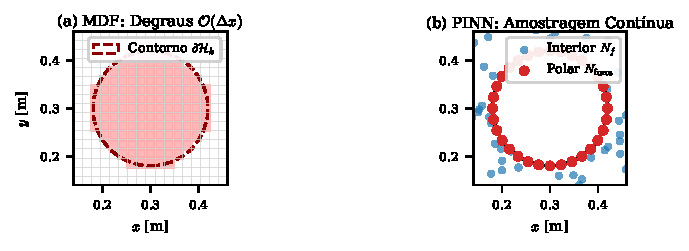
\includegraphics[width=0.60\textwidth]{figures/fig1_geometry_staircasing.pdf}\\
{\footnotesize Fonte: Elaboração própria.}
\end{figure}

Contudo, como ilustrado na Figura~\ref{fig:staircasing}(a), a presença das cavidades curvas $\partial\mathcal{H}_k$ impõe o erro de escadeamento (\textit{staircasing}), onde o contorno suave é aproximado por degraus ortogonais, degradando a acurácia dos fluxos normais $-\kappa \nabla u \cdot \mathbf{n}$ para $\mathcal{O}(\Delta x)$. Conforme examinado por \textcite{pereira2019}, correções por células de corte destroem a simetria direcional tridiagonal, impedindo o algoritmo de Thomas e elevando a complexidade para $\mathcal{O}(N^{1{,}5} \dots N^2)$.

\textbf{Arquitetura da PINN, Autograd e Retropropagação:} A formulação PINN de \textcite{raissi2019pinns} parametriza o campo contínuo $\hat{u}_\theta(x, y, t)$ por uma MLP profunda alimentada pelo vetor $\mathbf{z} = [x, y, t]^\top \in \mathbb{R}^3$, estruturada em $L = 5$ camadas ocultas com largura $d_h = 128$:
\begin{equation}
    \mathbf{h}_1 = \sigma\left(\mathbf{W}_1 \mathbf{z} + \mathbf{b}_1\right), \quad \mathbf{h}_\ell = \sigma\left(\mathbf{W}_\ell \mathbf{h}_{\ell-1} + \mathbf{b}_\ell\right), \quad \hat{u}_\theta(\mathbf{z}) = \mathbf{W}_{L+1} \mathbf{h}_L + b_{L+1},
\end{equation}
onde $\mathbf{W}_1 \in \mathbb{R}^{d_h \times 3}$, $\mathbf{b}_1 \in \mathbb{R}^{d_h}$; $\mathbf{W}_\ell \in \mathbb{R}^{d_h \times d_h}$, $\mathbf{b}_\ell \in \mathbb{R}^{d_h}$ ($\ell = 2, \dots, L$); e $\mathbf{W}_{L+1} \in \mathbb{R}^{1 \times d_h}$, $b_{L+1} \in \mathbb{R}$, totalizando $N_\theta = 66.689$ parâmetros treináveis com ativação $\sigma(z) = \tanh(z) \in C^\infty(\mathbb{R})$. O treinamento articula um duplo fluxo de gradientes: (i) a \textbf{diferenciação automática (\textit{autograd})} em relação a $\mathbf{z}$ avalia exatamente os termos da EDP $\frac{\partial \hat{u}_\theta}{\partial t}$ e $\nabla^2 \hat{u}_\theta = \frac{\partial^2 \hat{u}_\theta}{\partial x^2} + \frac{\partial^2 \hat{u}_\theta}{\partial y^2}$ por produtos vetor-Jacobiano sem malha; e (ii) o algoritmo de \textbf{retropropagação (\textit{backpropagation})} propaga o erro de $\mathcal{L}(\theta)$ pelas camadas para computar $\nabla_\theta \mathcal{L}(\theta)$ e atualizar os pesos sinápticos via otimização estocástica.

\subsection{Metodologia}

A amostragem de pontos colacionais opera diretamente sobre variedades analíticas contínuas (Figura~\ref{fig:staircasing}(b)): $N_f = 30.000$ pontos internos em $\Omega \times (0, T]$ ($24.000$ homogêneos e $6.000$ refinados na camada limite anular $r \in [r_k, r_k + 0{,}05]$); $N_{\mathrm{ic}} = 5.000$ pontos em $t=0$; $N_{\mathrm{ext}} = 8.000$ pontos em $\partial\Omega_{\mathrm{ext}} \times (0, T]$; e $N_{\mathrm{furos}} = 6.000$ pontos no contorno polar exato $\mathbf{x}_{\partial\mathcal{H}_k}(\theta_p) = (x_c^{(k)} + r_k \cos\theta_p, y_c^{(k)} + r_k \sin\theta_p)^\top$. O funcional multiobjetivo global ponderado $\mathcal{L}(\theta)$ é formulado na métrica $L_2$:
\begin{equation}
    \mathcal{L}(\theta) = \lambda_{\mathrm{pde}} \mathcal{L}_{\mathrm{pde}}(\theta) + \lambda_{\mathrm{ic}} \mathcal{L}_{\mathrm{ic}}(\theta) + \lambda_{\mathrm{ext}} \mathcal{L}_{\mathrm{ext}}(\theta) + \lambda_{\mathrm{furos}} \mathcal{L}_{\mathrm{furos}}(\theta),
\end{equation}
onde $\mathcal{L}_{\mathrm{pde}}$ penaliza o desvio da EDP via autograd, $\mathcal{L}_{\mathrm{ic}}$ impõe o repouso inicial, $\mathcal{L}_{\mathrm{ext}}$ assegura as bordas externas a $1{,}0$ e $\mathcal{L}_{\mathrm{furos}}$ impõe a barreira nula nos sumidouros. Adotam-se $\lambda_{\mathrm{ic}} = \lambda_{\mathrm{ext}} = 1{,}0$, $\lambda_{\mathrm{pde}} = 0{,}05$ e $\lambda_{\mathrm{furos}} = 2{,}0$. O treinamento estendeu-se por $50.000$ épocas em GPU (RTX 3050, $\approx 1{,}2$\,GB de VRAM, $104{,}2$ ms/época e $86{,}8$\,min totais) via Adam com Cosine Annealing ($\eta = 10^{-3} \to 10^{-5}$).

\subsection{Resultados e Discussão}

A Tabela~\ref{tab:perdas_finais} consolida os resíduos finais atingidos pela PINN após as 50.000 iterações.

\begin{table}[ht]
\caption{Métricas residuais finais da PINN na Equação do Calor 2D após 50.000 épocas.}
\label{tab:perdas_finais}
\centering
\small
\begin{tabular}{lccccc}
\toprule
\textbf{Componente} & $\mathcal{L}_{\mathrm{total}}$ & $\mathcal{L}_{\mathrm{pde}}$ & $\mathcal{L}_{\mathrm{ic}}$ & $\mathcal{L}_{\mathrm{ext}}$ & $\mathcal{L}_{\mathrm{furos}}$ \\
\midrule
\textbf{Valor Residual ($L_2$)} & $9{,}13 \times 10^{-3}$ & $8{,}56 \times 10^{-4}$ & $1{,}58 \times 10^{-4}$ & $2{,}51 \times 10^{-4}$ & $2{,}43 \times 10^{-6}$ \\
\bottomrule
\end{tabular}
\caption*{Fonte: Elaboração própria.}
\end{table}

\textbf{Convergência das Perdas, Rigidez Numérica e Relevo 3D ($t=2{,}0\,\mathrm{s}$):} A forte penalização de Dirichlet nas cavidades ($\lambda_{\mathrm{furos}} = 2{,}0$) induz matrizes Hessianas mal-condicionadas. A Figura~\ref{fig:loss_destaque}(a) detalha a trajetória das perdas ao longo das 50.000 iterações. Em vales estreitos da superfície de erro, as estimativas de momento do Adam acumulam inércia direcional em $\hat{m}_t$; próximo à época $26.000$, essa rigidez numérica impulsionou o estado contra paredes de alta curvatura, deflagrando uma oscilação transitória antes de restabelecer o decaimento estável. Em paralelo, a inspeção da solução contínua $\hat{u}_\theta \in C^\infty(\mathbb{R}^3)$ no estado avançado $t=2{,}0\,\mathrm{s}$ via projeção tridimensional de perfil (Figura~\ref{fig:loss_destaque}(b)) evidencia a formação de paredes íngremes de temperatura ao redor das cavidades dissipadoras, sustentando a barreira nula sob elevados gradientes térmicos.

\begin{figure}[!ht]
\centering
\caption{Diagnóstico de treinamento e relevo térmico: (a) dinâmica das componentes de perda da PINN com destaque para a rigidez numérica em 26k épocas; e (b) relevo tridimensional da chapa em $t=2{,}0\,\mathrm{s}$.}
\label{fig:loss_destaque}
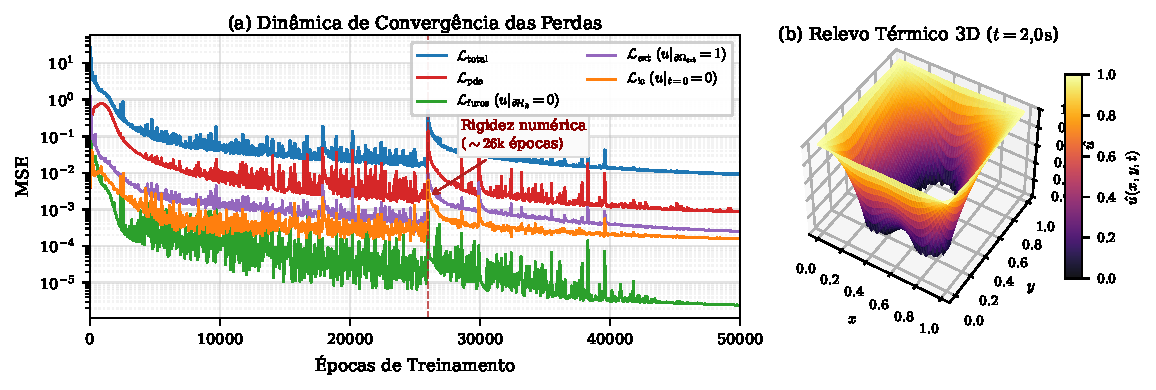
\includegraphics[width=0.98\textwidth]{figures/fig_loss_3d_duo.pdf}\\
{\footnotesize Fonte: Elaboração própria.}
\end{figure}

\textbf{Evolução Térmica Contínua e Falha na Extrapolação Temporal:} A Figura~\ref{fig:chapa_completa} ilustra o campo térmico completo em 6 instantes. Os painéis (a)--(e) exibem a difusão contínua do fluxo periférico quente e a retenção assintótica nos sumidouros em $t=0{,}05$, $0{,}2$, $0{,}5$, $1{,}0$ e $2{,}0$\,s. No painel (f), confirma-se o colapso físico sob extrapolação cega em $t=5{,}0$\,s devido à ausência de colocação além de $T=2{,}0$\,s.

\begin{figure}[!ht]
\centering
\caption{Evolução térmica espaço-temporal da chapa: (a--e) propagação transiente contínua em $t \in \{0{,}05;\, 0{,}20;\, 0{,}50;\, 1{,}00;\, 2{,}00\}\,\mathrm{s}$; e (f) colapso físico sob extrapolação temporal fora do horizonte treinado ($t=5{,}00\,\mathrm{s}$).}
\label{fig:chapa_completa}
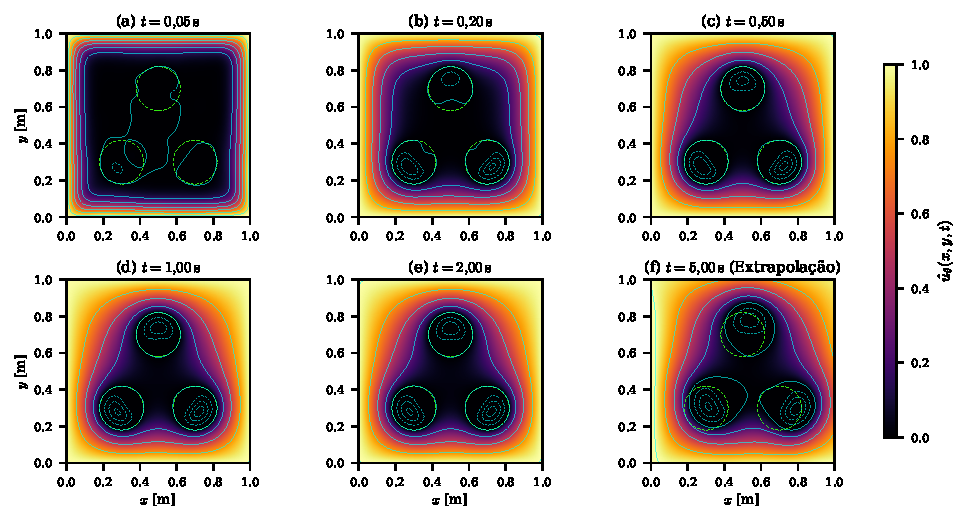
\includegraphics[width=0.71\textwidth]{figures/fig_combined_plate_analysis.pdf}\\
{\footnotesize Fonte: Elaboração própria.}
\end{figure}

\textbf{Comparativo Estrutural e Viés na Extrapolação Temporal:} A Tabela~\ref{tab:adi_vs_pinn} sumariza o confronto global entre os resolvedores. A PINN otimiza o domínio $\Omega \times [0, T]$ globalmente com inferências em $2{,}1$\,ms sem acumular erros pretéritos, mas colapsa para $t > T$, ao passo que o ADI \parencite{pereira2019} avança por marcha temporal causal indefinida.

\begin{table}[!ht]
\centering
\caption{Síntese comparativa: Método ADI \parencite{pereira2019} versus PINN contínua.}
\label{tab:adi_vs_pinn}
\footnotesize
\setlength{\tabcolsep}{2.5pt}
\begin{tabular}{lcc}
\toprule
\textbf{Critério de Avaliação} & \textbf{MDF ADI \parencite{pereira2019}} & \textbf{PINN (\textit{Meshless})} \\
\midrule
Discretização & Malha cartesiana $(\Delta x, \Delta y, \Delta t)$ & Espaço-tempo contínuo $\Omega \times [0, T]$ \\
Fronteiras Curvas ($\partial\mathcal{H}_k$) & Escadeamento $\mathcal{O}(\Delta x)$ & Amostragem polar analítica exata \\
Tempo de Processamento & Marcha ($85{,}4$\,ms / $2000$ passos) & Treinamento GPU ($86{,}8$\,min / $50\text{k}$ épocas) \\
Inferência Instantânea & Não aplicável (requer remarcha) & Avaliação direta ($2{,}1$\,ms para $\forall t \le T$) \\
Estabilidade & Incondicional ($L_2$ von Neumann) & Sujeita a rigidez de gradiente (\textit{stiffness}) \\
Extrapolação ($t > T$) & Marcha causal natural $t_{n+1} = t_n + \Delta t$ & Falha grave por perda de suporte \\
\bottomrule
\end{tabular}
\caption*{Fonte: Elaboração própria.}
\end{table}

\section{Considerações Finais}

A formulação PINN superou o erro de escadeamento e a perda da fatoração tridiagonal do método ADI em geometrias perfuradas, assegurando resíduo de $2{,}43 \times 10^{-6}$ nas barreiras Dirichlet dos sumidouros térmicos. A parametrização analítica via autograd dispensa malhas e viabiliza inferências instantâneas $\mathcal{O}(1)$. Contudo, constatou-se a sensibilidade do otimizador Adam à rigidez de gradiente em vales estreitos e o colapso na extrapolação temporal fora do suporte colacional. Enquanto o método ADI \parencite{pereira2019} sobressai na marcha temporal longa em domínios regulares, as PINNs consolidam-se como alternativa promissora para fronteiras irregulares complexas.

\renewcommand*{\bibfont}{\small}
\setlength{\bibitemsep}{2pt}
\begin{refcontext}[sorting=none]
\printbibliography
\end{refcontext}

\end{document}
